\documentclass[11pt]{article}

\usepackage[a4paper,margin=1in]{geometry}
\usepackage{amsmath,amssymb,amsfonts}
\usepackage{algorithm}
\usepackage{algorithmic}
\usepackage{graphicx}
\usepackage{booktabs}
\usepackage{hyperref}
\usepackage{xcolor}

\title{
Adaptive Multi-Resolution Grid-Based Clustering for Massive Data Streams
}

\author{
Alireza Zarei \\
Department of Mathematics and Computer Science \\
Sharif University of Technology \\
\texttt{zarei@sharif.ir}
% }
% \author{
\\
Mohammad Saleh Bahrami \\
Department of Mathematics and Computer Science \\
Sharif University of Technology \\
\texttt{saleh.bahrami98@sharif.edu}
}


\date{}

\begin{document}

\maketitle

\begin{abstract}
The rapid growth of streaming data generated by sensors, Internet of Things devices, online platforms, and scientific applications has created a need for clustering algorithms that can process data online under strict memory constraints. Grid-based density clustering methods, such as D-Stream, are attractive for data stream clustering because they summarize incoming points using grid cells instead of storing the entire stream. However, fixed-resolution grid methods suffer from two major limitations: their memory consumption grows rapidly with dimensionality, and a single global cell size may be unable to capture clusters with different local densities or evolving structures.

In this paper, we propose an adaptive multi-resolution grid-based framework for clustering massive data streams. The method maintains a hierarchical grid structure in which each cell stores compact statistical summaries, including time-decayed density, center of mass, variance, and update time. Cells are dynamically refined when their current resolution is insufficient to represent the local data distribution, and they are merged when high resolution is unnecessary or memory pressure increases. Sparse cells are periodically pruned to reduce memory usage. Clusters are extracted from dense connected grid regions using a density-based procedure inspired by DBSCAN.

The proposed framework improves the memory--accuracy trade-off of fixed-resolution grid-based stream clustering algorithms and provides a flexible mechanism for handling non-uniform data distributions and concept drift.
\end{abstract}

\noindent \textbf{Keywords:}
Data stream clustering; massive data; density-based clustering; grid-based clustering; multi-resolution grid; D-Stream; concept drift; memory-efficient algorithms.

\section{Introduction}

Massive data streams arise naturally in many modern applications, including sensor networks, Internet of Things systems, financial transactions, web logs, network monitoring, and computational biology. In such settings, data points arrive continuously and potentially without bound. Therefore, traditional clustering algorithms, which assume that the entire dataset is stored in memory and can be processed multiple times, are often infeasible.

The data stream model imposes two important constraints. First, the algorithm must process each data point online, usually in one pass. Second, the available memory is significantly smaller than the size of the stream. As a result, stream clustering algorithms typically maintain a compact summary of the observed data rather than storing all incoming points.

Clustering is one of the fundamental tasks in unsupervised learning and data mining. Its goal is to group similar objects together while separating dissimilar objects. Among different clustering approaches, density-based methods are especially useful because they can detect clusters of arbitrary shape and distinguish noise or outliers from meaningful dense regions. However, applying density-based clustering directly to data streams is challenging because density estimates must be updated continuously and efficiently.

Grid-based density clustering methods address this challenge by partitioning the data space into cells and maintaining density summaries for these cells. A well-known example is D-Stream, which uses a fixed-resolution grid and a fading function to give more importance to recent data. Although such methods are efficient, they suffer from important limitations. The number of cells grows exponentially with the dimension of the data, and a fixed grid resolution may be inappropriate for data whose density varies across space or changes over time.

To address these limitations, this paper proposes an adaptive multi-resolution grid-based clustering framework for massive data streams. Instead of using a single global grid resolution, the proposed method dynamically refines or merges grid cells according to local statistical properties of the stream and the available memory budget. Dense or complex regions can be represented by smaller cells, while sparse or simple regions can be summarized by larger cells.

The main idea is to maintain a hierarchical grid structure, such as a quadtree in two dimensions or a $2^d$-tree in $d$ dimensions. Each cell stores a compact feature vector describing the local data distribution. Based on this vector, the algorithm decides whether the cell should be refined, merged, pruned, or kept unchanged.

\subsection{Contributions}

The main contributions of this paper are as follows:

\begin{itemize}
    \item We propose an adaptive multi-resolution grid framework for density-based clustering of massive data streams.
    
    \item We introduce dynamic refinement and contraction operations that allow the grid resolution to change over both space and time.
    
    \item We maintain compact cell-level summaries, including time-decayed density, center of mass, variance, and update time, to guide refinement and merging decisions.
    
    \item We incorporate sparse-cell pruning to reduce memory consumption and remove cells that have negligible influence on clustering quality.
    
    \item We describe a density-based clustering procedure over active grid cells, reducing the need to cluster raw data points.
    
    \item We provide a framework that can be viewed as an adaptive multi-resolution extension of fixed-grid stream clustering algorithms such as D-Stream.
\end{itemize}

\section{Related Work}

Data stream clustering has been widely studied due to the increasing importance of real-time data analysis. Existing methods can be broadly categorized into micro-cluster-based methods, density-based methods, grid-based methods, and hybrid approaches.

CluStream is one of the early frameworks for clustering data streams. It separates the process into an online micro-clustering phase and an offline macro-clustering phase. DenStream extends the micro-cluster idea using density-based potential and outlier micro-clusters. DBSTREAM also follows a density-based strategy and maintains shared density information between micro-clusters.

Grid-based methods partition the data space into cells and maintain summaries for these cells. STING is an early statistical grid-based method that stores statistical information in hierarchical grid cells. D-Stream adapts grid-based clustering to data streams by using a density decay factor and periodically removing sparse grids. These methods are efficient, but their performance depends heavily on the choice of grid resolution.

The main weakness of fixed-grid approaches is that one global cell size cannot represent all regions of a non-uniform or evolving data stream equally well. If the cell size is too large, distinct clusters may be merged. If the cell size is too small, the number of cells may become too large, causing high memory consumption and computational overhead.

Our method is motivated by these limitations. It combines the compact representation of grid-based methods, the time-decayed density mechanism of D-Stream, the statistical summaries of STING-like methods, and the sparse-cell pruning philosophy of stream clustering algorithms such as CEDAS.

\section{Problem Definition}

Let
\[
X = \{x_1, x_2, \ldots, x_t, \ldots\}
\]
be a data stream, where each point $x_t \in \mathbb{R}^d$ arrives at time $t$. The stream may be very large or potentially infinite, so the algorithm cannot store all points.

The goal is to maintain, at any time $t$, a clustering of the points observed so far, or more precisely, a clustering of their compact summaries. The algorithm should satisfy the following requirements:

\begin{itemize}
    \item It should process each point online.
    \item It should use memory significantly smaller than the number of observed points.
    \item It should adapt to changes in the data distribution.
    \item It should detect clusters of arbitrary shape.
    \item It should handle noise and sparse regions efficiently.
\end{itemize}

\subsection{Time-Decayed Density}

Following D-Stream, we assign higher importance to recent data points. Let $\lambda \in (0,1)$ be a decay factor. If a point $x_i$ arrived at time $T(x_i)$, its density contribution at time $t$ is defined as
\[
D(x_i,t) = \lambda^{t - T(x_i)}.
\]

For a grid cell $g$, the time-decayed density at time $t$ is
\[
D(g,t) = \sum_{x_i \in E(g,t)} \lambda^{t - T(x_i)},
\]
where $E(g,t)$ is the set of points assigned to cell $g$ before or at time $t$.

If the last update time of cell $g$ is $t_l$ and a new point arrives at time $t_n$, the density can be updated efficiently by
\[
D(g,t_n) = \lambda^{t_n - t_l} D(g,t_l) + 1.
\]

This update requires constant time for the affected cell.

\section{Proposed Method}

The proposed method maintains an adaptive hierarchical grid. Unlike fixed-resolution grid methods, different regions of the data space may be represented at different resolutions.

\subsection{Hierarchical Grid Structure}

The data space is initially represented by a coarse grid. Each grid cell may be recursively divided into smaller child cells. In two dimensions, this structure corresponds to a quadtree. In $d$ dimensions, each refinement divides a cell into $2^d$ child cells.

Each cell $g$ has a level $\ell(g)$, where lower levels correspond to coarser cells and higher levels correspond to finer cells. The side length of a cell at level $\ell$ is denoted by $h_\ell$.

\subsection{Cell Summary}

Each active cell stores a compact summary vector:
\[
\Phi(g) =
\left(
D(g), \mu(g), \sigma^2(g), t_g, \ell(g), n(g)
\right),
\]
where:

\begin{itemize}
    \item $D(g)$ is the time-decayed density of the cell,
    \item $\mu(g)$ is the time-decayed center of mass,
    \item $\sigma^2(g)$ is the estimated variance,
    \item $t_g$ is the last update time,
    \item $\ell(g)$ is the cell level,
    \item $n(g)$ is the number of points or weighted count assigned to the cell.
\end{itemize}

The center of mass can be updated online. If a new point $x_t$ is assigned to cell $g$, then after applying decay to the previous statistics, the updated center can be computed as
\[
\mu(g,t) =
\frac{
\lambda^{t-t_g}D(g,t_g)\mu(g,t_g) + x_t
}{
\lambda^{t-t_g}D(g,t_g) + 1
}.
\]

Similar online updates can be used for the variance.

\subsection{Refinement Criterion}
\label{sec:proposed-method-refinement}

A cell should be refined when its current resolution is not sufficient to represent the local data distribution. We define a refinement score:
\[
R(g) =
\alpha_1 \cdot \frac{\sigma^2(g)}{h_{\ell(g)}^2}
+
\alpha_2 \cdot
\frac{\|\mu(g) - c(g)\|^2}{h_{\ell(g)}^2}
+
\alpha_3 \cdot \rho(g),
\]
where:

\begin{itemize}
    \item $c(g)$ is the geometric center of the cell,
    \item $h_{\ell(g)}$ is the side length of the cell,
    \item $\rho(g)$ is an optional local density irregularity measure,
    \item $\alpha_1,\alpha_2,\alpha_3$ are weighting parameters.
\end{itemize}

The intuition is as follows. If the variance inside a cell is large, or if the center of mass is far from the geometric center, then the assumption that data is uniformly distributed inside the cell may be inaccurate. In such cases, the cell may need to be refined.

A cell $g$ is refined if
\[
R(g) > \tau_{\text{split}},
\]
provided that the memory budget allows refinement and the maximum grid depth has not been reached.

\subsection{Contraction Criterion}

The algorithm may merge child cells into their parent when high resolution is unnecessary. Let $g_1,\ldots,g_{2^d}$ be the children of a parent cell $p$. These children can be merged if their combined representation is sufficiently close to the parent-level approximation.

A possible contraction condition is
\[
\max_i R(g_i) < \tau_{\text{merge}},
\]
or
\[
\Delta(p) < \epsilon_{\text{merge}},
\]
where $\Delta(p)$ measures the information loss caused by replacing the children with their parent.

Contraction is especially useful when memory usage approaches the allowed memory budget.

\subsection{Sparse Cell Pruning}

Cells with very low decayed density are unlikely to contribute significantly to the final clustering. Therefore, the algorithm periodically removes sparse cells.

A cell $g$ is pruned if
\[
D(g,t) < \tau_{\text{sparse}},
\]
and it has not received new points for a sufficiently long time.

This pruning mechanism reduces memory usage and allows the algorithm to focus on active dense regions of the stream.

\subsection{Clustering over Grid Cells}

At query time or after a fixed number of updates, the algorithm extracts clusters from the active grid cells.

Each active cell is labeled as:

\begin{itemize}
    \item \textbf{dense}, if $D(g,t) \geq \tau_{\text{dense}}$,
    \item \textbf{transitional}, if $\tau_{\text{sparse}} \leq D(g,t) < \tau_{\text{dense}}$,
    \item \textbf{sparse}, if $D(g,t) < \tau_{\text{sparse}}$.
\end{itemize}

A graph is constructed over dense cells. Two cells are connected if they are spatial neighbors and their resolutions are compatible. Clusters are then obtained as connected components of this graph. Transitional cells may be assigned to nearby dense clusters if they satisfy a neighborhood condition.

This procedure is similar in spirit to DBSCAN, but it operates on grid cells rather than raw data points.

\section{Algorithm}

\begin{algorithm}[t]
\caption{Adaptive Multi-Resolution Grid Stream Clustering}
\label{alg:adaptive-grid}
\begin{algorithmic}[1]
\STATE Initialize root grid cells.
\STATE Set decay factor $\lambda$, thresholds $\tau_{\text{split}}$, $\tau_{\text{merge}}$, $\tau_{\text{sparse}}$, and memory budget $M$.
\FOR{each incoming point $x_t$}
    \STATE Locate the finest active cell $g$ containing $x_t$.
    \STATE Apply time decay to the statistics of $g$.
    \STATE Update $D(g)$, $\mu(g)$, $\sigma^2(g)$, and $t_g$.
    \IF{$R(g) > \tau_{\text{split}}$ and memory usage is below $M$}
        \STATE Refine $g$ into $2^d$ child cells.
        \STATE Distribute the summary of $g$ among its children using the available cell statistics.
    \ENDIF
    \IF{memory usage is close to $M$}
        \STATE Increase refinement strictness.
        \STATE Attempt contraction of low-information child cells.
    \ENDIF
    \IF{pruning condition is triggered}
        \STATE Remove cells with $D(g,t) < \tau_{\text{sparse}}$.
    \ENDIF
\ENDFOR
\STATE Extract clusters from connected dense cells.
\end{algorithmic}
\end{algorithm}

\section{Complexity Analysis}

Let $m$ be the number of active cells currently stored by the algorithm. Since the algorithm does not store all observed points, its memory complexity is
\[
O(m),
\]
where $m$ is controlled by the memory budget and pruning mechanism.

For each incoming point, the algorithm must locate the corresponding active cell and update its summary. If the hierarchical grid has maximum depth $L$, then point insertion requires
\[
O(L)
\]
time in the worst case. For fixed maximum depth, this becomes constant or logarithmic in the number of active cells depending on the implementation.

The refinement of a cell creates $2^d$ children. Therefore, the cost of a refinement operation is
\[
O(2^d).
\]
However, refinement is not performed for every point and is controlled by the refinement threshold and memory budget.

The clustering phase operates over active dense cells. If $m_d$ is the number of dense cells, then constructing the adjacency graph and finding connected components requires approximately
\[
O(m_d \cdot \eta),
\]
where $\eta$ is the number of neighboring cells checked for each cell. In fixed dimension, $\eta$ is usually bounded by a constant.

\section{Experimental Evaluation}

To evaluate the proposed method, it should be compared against representative stream clustering algorithms, including D-Stream, DenStream, CluStream, DBSTREAM, and CEDAS.

\subsection{Datasets}

The experimental evaluation may include both synthetic and real-world datasets.

Synthetic datasets are useful because they allow controlled testing of:

\begin{itemize}
    \item varying cluster densities,
    \item arbitrary cluster shapes,
    \item noise and outliers,
    \item concept drift,
    \item high-dimensional behavior.
\end{itemize}

Real-world datasets may include sensor data, network traffic data, GPS trajectories, or IoT streams.

\subsection{Evaluation Metrics}

The following metrics can be used:

\begin{itemize}
    \item Adjusted Rand Index,
    \item Normalized Mutual Information,
    \item clustering purity,
    \item silhouette score,
    \item memory usage,
    \item processing time per point,
    \item throughput,
    \item number of active cells,
    \item robustness to concept drift.
\end{itemize}

\subsection{Expected Results}

The proposed method is expected to use less memory than fixed-resolution grid methods in sparse or non-uniform data streams. It is also expected to produce better clustering accuracy when clusters have different densities or when a fixed grid resolution is inappropriate. Section~\ref{sec:results} reports the empirical outcome of testing this expectation against a first working prototype.

\section{Results}
\label{sec:results}

This section reports results from a v0 research prototype of the proposed method, implemented in Python, and compared against a swept fixed-resolution D-Stream baseline and three imported reference methods. We report these results as an honest snapshot of an early-stage implementation rather than a demonstration of a finished method: the prototype is currently dominated by the baselines, and we identify two concrete, verified causes for the gap.

\subsection{Experimental Setup}

We use a synthetic two-dimensional stream, \texttt{varying\_density} (seed 7, $n=4000$ points), constructed so that a single fixed grid resolution provably cannot represent both clusters well: a tight, dense Gaussian cluster ($\sigma = 0.18$) and a broad, sparse Gaussian cluster ($\sigma = 1.6$) are present simultaneously throughout the stream, with both centers drifting across three phases. Models are evaluated prequentially, that is, each incoming point is scored against the model's current state before the model is updated on it.

The reference frontier is a fixed-resolution D-Stream swept over ten grid resolutions, $n_{\text{cells per dim}} \in \{2,3,4,6,8,11,16,22,32,45\}$, tracing out an accuracy-versus-memory curve rather than a single operating point. We additionally import three published stream clustering methods from the \texttt{river} library, DenStream, CluStream, and DBSTREAM, without modification, so that the adaptive method is compared against real published baselines and not only against a self-authored fixed-grid ablation. Peak memory is measured with \texttt{tracemalloc} from before model construction, so that a fixed grid's upfront cell allocation is counted rather than only the cost of the online update phase. Points that fall in a non-dense cell are assigned a sentinel label rather than being dropped, so that a model which abstains on much of the stream is not rewarded for doing so.

\subsection{Accuracy--Memory Frontier in Two Dimensions}

Table~\ref{tab:frontier} reports peak memory, Adjusted Rand Index (ARI), Normalized Mutual Information (NMI), and the fraction of unassigned points for the fixed-grid frontier, the three imported baselines, and the adaptive method. Figure~\ref{fig:frontier} plots ARI and NMI against peak memory for all models.

\begin{table}[h]
\centering
\caption{Accuracy--memory frontier on the varying-density stream (2D, $n=4000$, seed 7). AdaptiveDStream is highlighted; it is dominated on both axes by the fixed-grid frontier at comparable memory and by every imported baseline.}
\label{tab:frontier}
\begin{tabular}{lrrrr}
\toprule
Model & Peak memory (KB) & ARI & NMI & Frac.\ unassigned \\
\midrule
FixedGrid $n{=}2$   & 7.4    & 0.000 & 0.008 & 0.00 \\
FixedGrid $n{=}4$   & 18.2   & 0.002 & 0.045 & 0.03 \\
FixedGrid $n{=}8$   & 54.3   & 0.048 & 0.148 & 0.11 \\
DBSTREAM            & 25.6   & 0.166 & 0.172 & 0.00 \\
FixedGrid $n{=}11$  & 97.2   & 0.093 & 0.152 & 0.19 \\
DenStream           & 73.6   & 0.128 & 0.261 & 0.00 \\
CluStream           & 102.1  & 0.037 & 0.042 & 0.00 \\
FixedGrid $n{=}16$  & 199.4  & 0.299 & 0.274 & 0.36 \\
FixedGrid $n{=}22$  & 376.9  & 0.474 & 0.414 & 0.46 \\
FixedGrid $n{=}32$  & 793.2  & 0.614 & 0.551 & 0.53 \\
\textbf{AdaptiveDStream} & \textbf{1344.3} & \textbf{0.106} & \textbf{0.107} & \textbf{0.42} \\
FixedGrid $n{=}45$  & 1568.1 & 0.726 & 0.650 & 0.55 \\
\bottomrule
\end{tabular}
\end{table}

\begin{figure}[h]
\centering
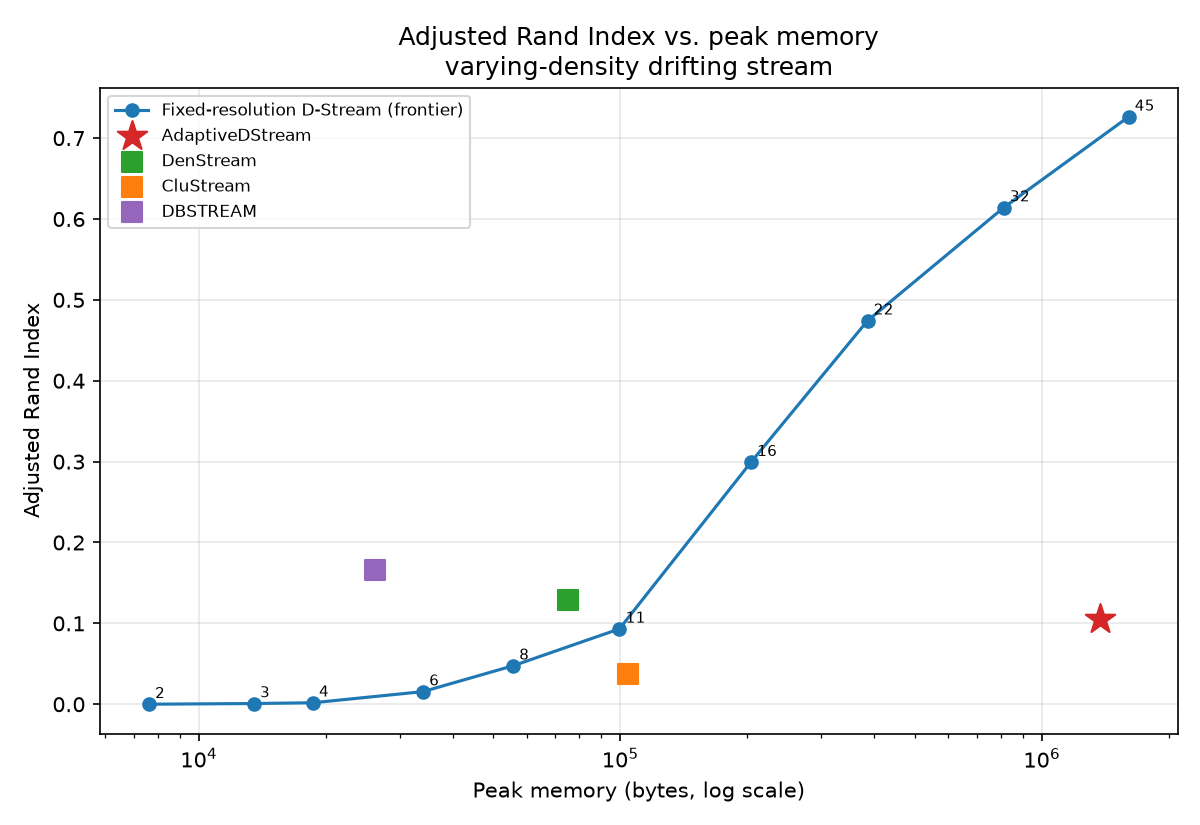
\includegraphics[width=0.48\textwidth]{figures/frontier_ari_vs_memory.png}
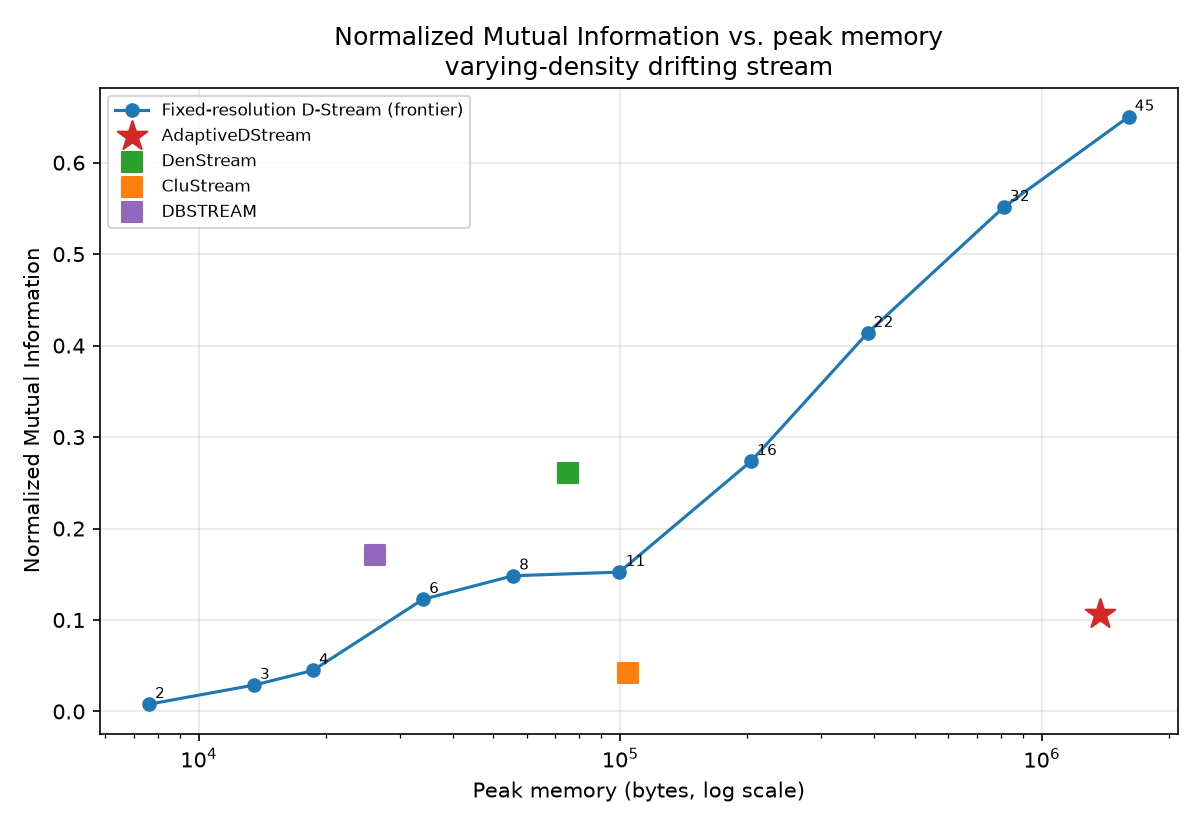
\includegraphics[width=0.48\textwidth]{figures/frontier_nmi_vs_memory.png}
\caption{ARI (left) and NMI (right) versus peak memory for the fixed-grid frontier, the three imported baselines, and AdaptiveDStream.}
\label{fig:frontier}
\end{figure}

At its own memory footprint (1344 KB, between the fixed grids at $n{=}32$ and $n{=}45$), the fixed-grid frontier reaches ARI 0.61--0.73, versus 0.106 for the adaptive method. The adaptive method is also beaten simultaneously on both axes by every imported baseline: DBSTREAM reaches higher ARI (0.166) using roughly 50 times less memory (25.6~KB). We report this as the current, unvarnished result of the prototype rather than omit it: on this stream, the v0 implementation is not yet competitive.

\subsection{Root-Cause Analysis of the Accuracy Gap}
\label{sec:root-cause}

We traced the gap to two specific, verified implementation issues, both concerning how the dense/sparse rule and memory accounting interact with splitting, rather than the splitting heuristic (when to split) itself.

\begin{enumerate}
    \item \textbf{The dense threshold is an absolute decayed count, not a density.} Splitting a cell fragments its accumulated mass across its $2^d$ children. A region can be genuinely dense, that is, have high mass per unit volume, while every fine cell covering it holds too little raw decayed count to cross $\tau_{\text{dense}}$, simply because the same mass is now divided among more cells. Consequently no single absolute threshold value is correct both before and after a region is refined. We verified this is the dominant effect by manually sweeping the threshold pair from $(\tau_{\text{dense}}, \tau_{\text{sparse}}) = (2.0, 0.3)$, the value shared with the fixed-grid baseline, down to $(0.5, 0.05)$: ARI improved from 0.040 to only about 0.106 before plateauing, never approaching the fixed-grid frontier. This matches the original D-Stream formulation, which compares density, count divided by cell volume, against a threshold; the prototype currently omits the volume normalization.
    \item \textbf{Splitting does not free the parent cell's storage.} The split operation attaches $2^d$ children to a cell but leaves the parent object itself resident in memory, still referenced by its own parent and still holding its sufficient statistics. In the run underlying Table~\ref{tab:frontier}, the model ended with 1309 leaf cells, which implies exactly $(1309-1)/3 = 436$ split events and therefore $1309 + 436 = 1745$ live cell objects in total, as much memory as a $42 \times 42$ fixed grid rather than the $36 \times 36$ grid that the leaf count alone would suggest. Roughly a quarter of the adaptive method's reported memory in this run is retired parent cells that no longer participate in lookup or clustering.
\end{enumerate}

Both issues point toward the same fix: making the dense/sparse classification and the memory accounting resolution-aware, rather than revising the criterion that decides \emph{when} to split.

\subsection{Effect of Dimensionality}
\label{sec:dim-sweep}

We repeated the comparison on the same stream family generalized to $d > 2$, with the two cluster centers orbiting in the first two coordinates and every additional dimension carrying pure isotropic noise, the standard curse-of-dimensionality stress case. This is a preliminary probe rather than a full multi-dimensional evaluation: it uses a single seed, $n = 2500$ points, and neither model's thresholds were retuned per dimension. At each dimension, the fixed grid's resolution was chosen so its total cell count lands near the adaptive method's $2500$-cell budget, so the comparison is roughly memory-matched rather than resolution-matched. Table~\ref{tab:dimsweep} and Figure~\ref{fig:dimsweep} summarize the outcome for $d \in \{2,3,4,5,6,8,10\}$.

\begin{table}[h]
\centering
\caption{Effect of dimensionality on peak memory and accuracy, at roughly matched memory budgets (varying-density stream, $n=2500$, seed 7, single run per dimension).}
\label{tab:dimsweep}
\begin{tabular}{rlrrrr}
\toprule
Dim & Model & Cells & Peak memory (KB) & ARI & NMI \\
\midrule
2  & FixedGrid ($n{=}50$) & 2500 & 1930.8 & 0.627 & 0.577 \\
2  & \textbf{AdaptiveDStream} & 850  & \textbf{870.7}  & 0.074 & 0.104 \\
3  & FixedGrid ($n{=}14$) & 2744 & 2200.3 & 0.653 & 0.629 \\
3  & \textbf{AdaptiveDStream} & 1296 & \textbf{1183.9} & 0.015 & 0.057 \\
4  & FixedGrid ($n{=}7$)  & 2401 & 2002.0 & 0.465 & 0.418 \\
4  & \textbf{AdaptiveDStream} & 1966 & \textbf{1742.7} & 0.020 & 0.073 \\
5  & FixedGrid ($n{=}5$)  & 3125 & 2701.2 & 0.496 & 0.476 \\
5  & \textbf{AdaptiveDStream} & 2481 & \textbf{2205.4} & 0.050 & 0.096 \\
6  & FixedGrid ($n{=}4$)  & 4096 & 3666.8 & 0.328 & 0.308 \\
6  & \textbf{AdaptiveDStream} & 2458 & \textbf{2227.1} & 0.043 & 0.076 \\
8  & FixedGrid ($n{=}3$)  & 6561 & 6284.7 & 0.520 & 0.511 \\
8  & \textbf{AdaptiveDStream} & 2296 & \textbf{2205.4} & 0.210 & 0.185 \\
10 & FixedGrid ($n{=}2$)  & 1024 & 1047.6 & 0.486 & 0.495 \\
10 & \textbf{AdaptiveDStream} & 2047 & \textbf{2093.0} & 0.291 & 0.258 \\
\bottomrule
\end{tabular}
\end{table}

\begin{figure}[h]
\centering
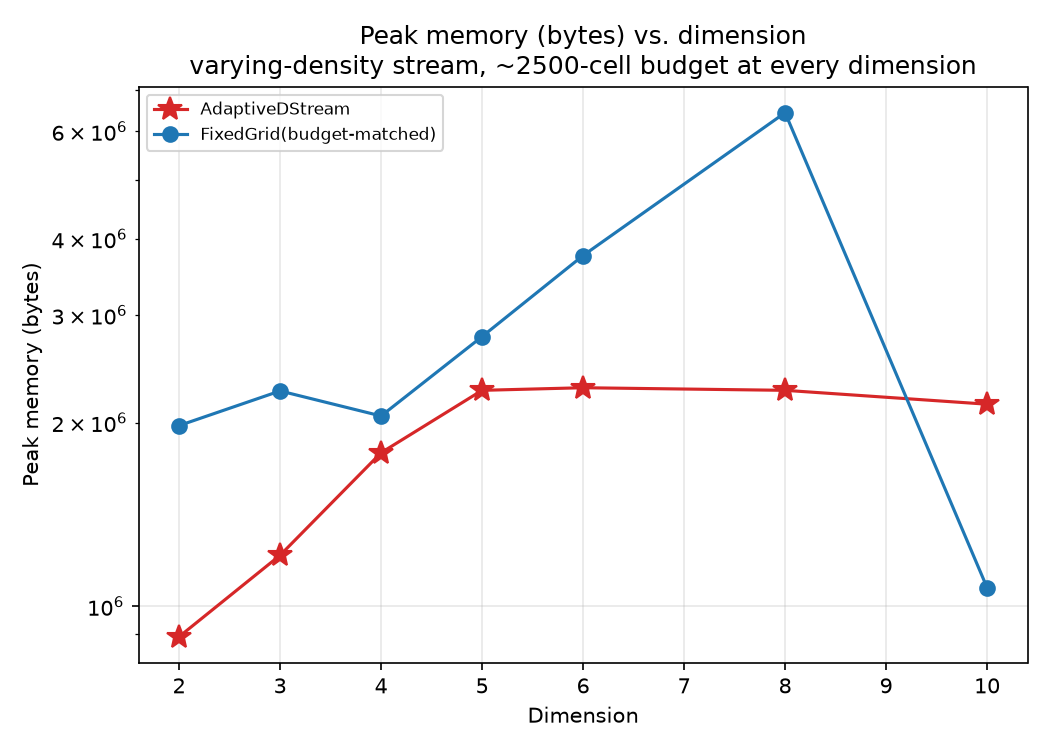
\includegraphics[width=0.48\textwidth]{figures/dimension_sweep_memory.png}
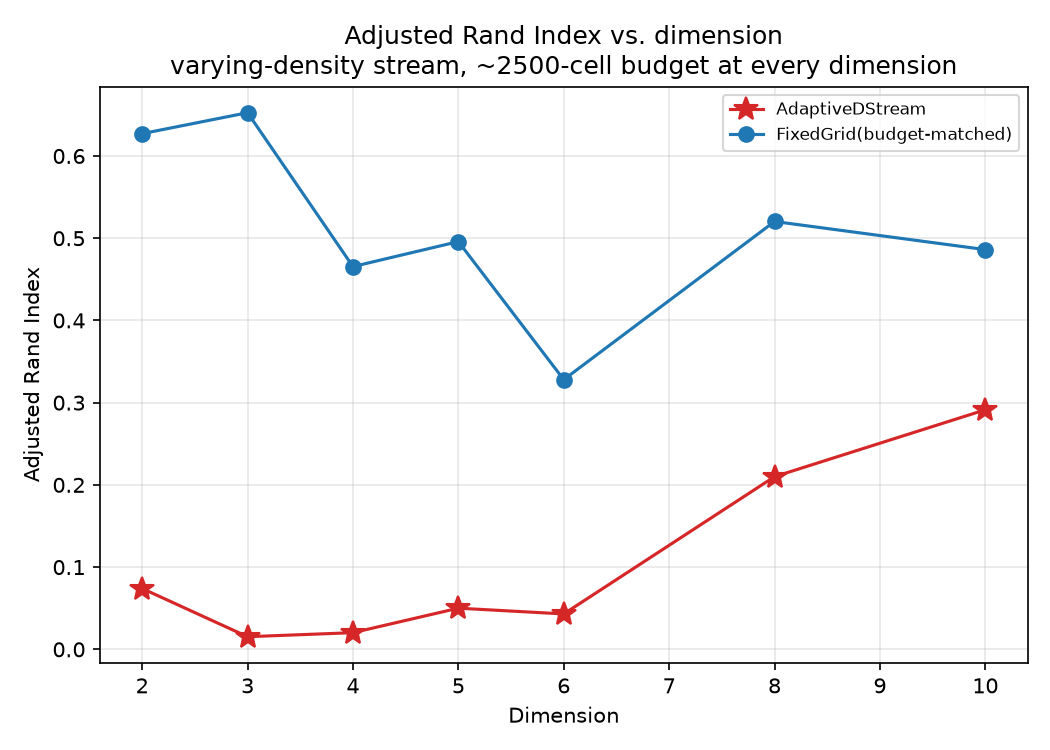
\includegraphics[width=0.48\textwidth]{figures/dimension_sweep_ari.png}
\caption{Peak memory (left) and ARI (right) versus dimension, comparing AdaptiveDStream against a fixed grid whose resolution is chosen to match its cell budget at each dimension.}
\label{fig:dimsweep}
\end{figure}

Two patterns emerge. First, the memory hypothesis behind the method is partially supported: from $d=2$ to $d=8$, AdaptiveDStream uses only 35--87\% of the budget-matched fixed grid's memory and plateaus near its $\texttt{max\_cells}$ cap, while the fixed grid's memory keeps climbing because its cell count scales as $n_{\text{cells per dim}}^d$ and, at high dimension, $n_{\text{cells per dim}}$ can only move in coarse integer steps: at $d=8$, going from $n=2$ (256 cells) to $n=3$ (6561 cells) overshoots the 2500-cell target by 2.6$\times$ with no intermediate resolution available. Past a point, a fixed grid is not just more expensive in high dimension, it stops being tunable to a given memory budget at all.

Second, AdaptiveDStream remains dominated in accuracy at every dimension tested, consistent with the root cause identified in Section~\ref{sec:root-cause}: a fixed, non-volume-normalized dense threshold is penalized more harshly as dimension grows, since a split fragments mass across $2^d$ children, a 256-way fragmentation at $d=8$ versus 4-way at $d=2$. The relative gap does narrow at high dimension, from 2--13\% of the fixed grid's ARI at $d=2$--$6$ to 40\% at $d=8$ and 60\% at $d=10$, but part of this narrowing is the fixed-grid baseline itself degrading as uninformative noise dimensions dilute Euclidean-adjacency clustering, not only AdaptiveDStream improving. Given the single seed, untuned per-dimension thresholds, and smaller sample size used here, we treat this dimensionality result as a preliminary signal worth pursuing rather than a validated finding.

\subsection{Summary of Findings}

The current prototype is not yet competitive with either the fixed-grid frontier or the imported published baselines on the evaluated stream. We consider this an honest characterization of a first working implementation rather than a limitation of the underlying idea: both identified causes are implementation choices, an absolute rather than volume-normalized density threshold, and unreclaimed memory from split parent cells, that are independent of the refinement criterion itself (Section~\ref{sec:proposed-method-refinement}). The dimensionality experiment additionally shows that the method's memory footprint does scale more gracefully than a fixed grid's, supporting one half of the original motivation, while accuracy parity remains an open problem. Addressing the two root causes above and re-running this evaluation is the immediate next step, ahead of any change to the splitting heuristic itself.

\section{Discussion}

The proposed framework addresses a central limitation of fixed-grid stream clustering algorithms: the inability to adapt the grid resolution to local data complexity. By refining only complex or dense regions and merging simple or sparse regions, the algorithm provides a practical trade-off between clustering accuracy and memory consumption.

The use of time-decayed density makes the method suitable for evolving streams. Older data gradually loses influence, allowing the clustering structure to adapt to recent patterns. Moreover, sparse-cell pruning prevents the algorithm from wasting memory on inactive regions.

However, the method also introduces new challenges. The refinement and merging thresholds must be chosen carefully. If refinement is too aggressive, memory usage may grow quickly. If refinement is too conservative, clusters may be represented too coarsely. Adaptive threshold selection is therefore an important direction for future work.

\section{Conclusion}

This paper proposed an adaptive multi-resolution grid-based framework for clustering massive data streams. The method extends fixed-resolution grid-based approaches by allowing grid cells to be dynamically refined, merged, and pruned according to local statistical summaries and memory constraints. Each cell stores compact information such as time-decayed density, center of mass, and variance. Clusters are extracted from connected dense cells using a density-based procedure.

The proposed approach is designed to improve the memory--accuracy trade-off of grid-based stream clustering methods and to better handle non-uniform, evolving data streams. Future work includes developing stronger theoretical guarantees, incorporating dimensionality reduction, improving concept drift detection, and performing extensive experimental comparison with existing stream clustering algorithms.

\section*{Future Work}

Several extensions can further improve the proposed framework:

\begin{itemize}
    \item \textbf{Streaming dimensionality reduction:} Random projections, incremental PCA, or streaming autoencoders can be used before grid construction to reduce the effect of high dimensionality.
    
    \item \textbf{Adaptive threshold learning:} The refinement, merging, and pruning thresholds can be adjusted automatically based on memory pressure, density variation, or clustering stability.
    
    \item \textbf{Explicit concept drift detection:} Drift detectors such as ADWIN, Page-Hinkley, DDM, or EDDM can be incorporated to trigger refinement or reorganization of the grid.
    
    \item \textbf{Sketch-based summaries:} Count-Min Sketch, reservoir sampling, or exponential histograms can be used to improve the accuracy of cell-level summaries.
    
    \item \textbf{Incremental connectivity maintenance:} Instead of recomputing clusters from scratch, dynamic graph connectivity or union-find structures can maintain clusters over dense cells incrementally.
    
    \item \textbf{Distributed and GPU implementations:} The grid update and clustering steps can be parallelized for high-throughput data streams.
\end{itemize}

\bibliographystyle{plain}
\begin{thebibliography}{99}

\bibitem{Aggarwal2003CluStream}
C. C. Aggarwal, J. Han, J. Wang, and P. S. Yu.
A framework for clustering evolving data streams.
In \textit{Proceedings of the International Conference on Very Large Data Bases}, 2003.

\bibitem{Aggarwal2007DataStreams}
C. C. Aggarwal.
\textit{Data Streams: Models and Algorithms}.
Springer, 2007.

\bibitem{Cao2006DenStream}
F. Cao, M. Ester, W. Qian, and A. Zhou.
Density-based clustering over an evolving data stream with noise.
In \textit{Proceedings of the SIAM International Conference on Data Mining}, 2006.

\bibitem{Chen2007DStream}
Y. Chen and L. Tu.
Density-based clustering for real-time stream data.
In \textit{Proceedings of the ACM SIGKDD International Conference on Knowledge Discovery and Data Mining}, 2007.

\bibitem{Ester1996DBSCAN}
M. Ester, H.-P. Kriegel, J. Sander, and X. Xu.
A density-based algorithm for discovering clusters in large spatial databases with noise.
In \textit{Proceedings of the International Conference on Knowledge Discovery and Data Mining}, 1996.

\bibitem{Hahsler2016DBSTREAM}
M. Hahsler and M. Bola{\~n}os.
Clustering data streams based on shared density between micro-clusters.
\textit{IEEE Transactions on Knowledge and Data Engineering}, 2016.

\bibitem{Hyde2017CEDAS}
R. Hyde, P. Angelov, and A. R. MacKenzie.
Fully online clustering of evolving data streams into arbitrarily shaped clusters.
\textit{Information Sciences}, 2017.

\bibitem{Wang1997STING}
W. Wang, J. Yang, and R. Muntz.
STING: A statistical information grid approach to spatial data mining.
In \textit{Proceedings of the International Conference on Very Large Data Bases}, 1997.

\end{thebibliography}

\end{document}
